\section{Tools}

\section{Simulation Design}

Figure \ref{fig:simulation_design} shows the general simulation setup that is used to test the software components of the proposed system.

\begin{figure}[h]
	\centering
		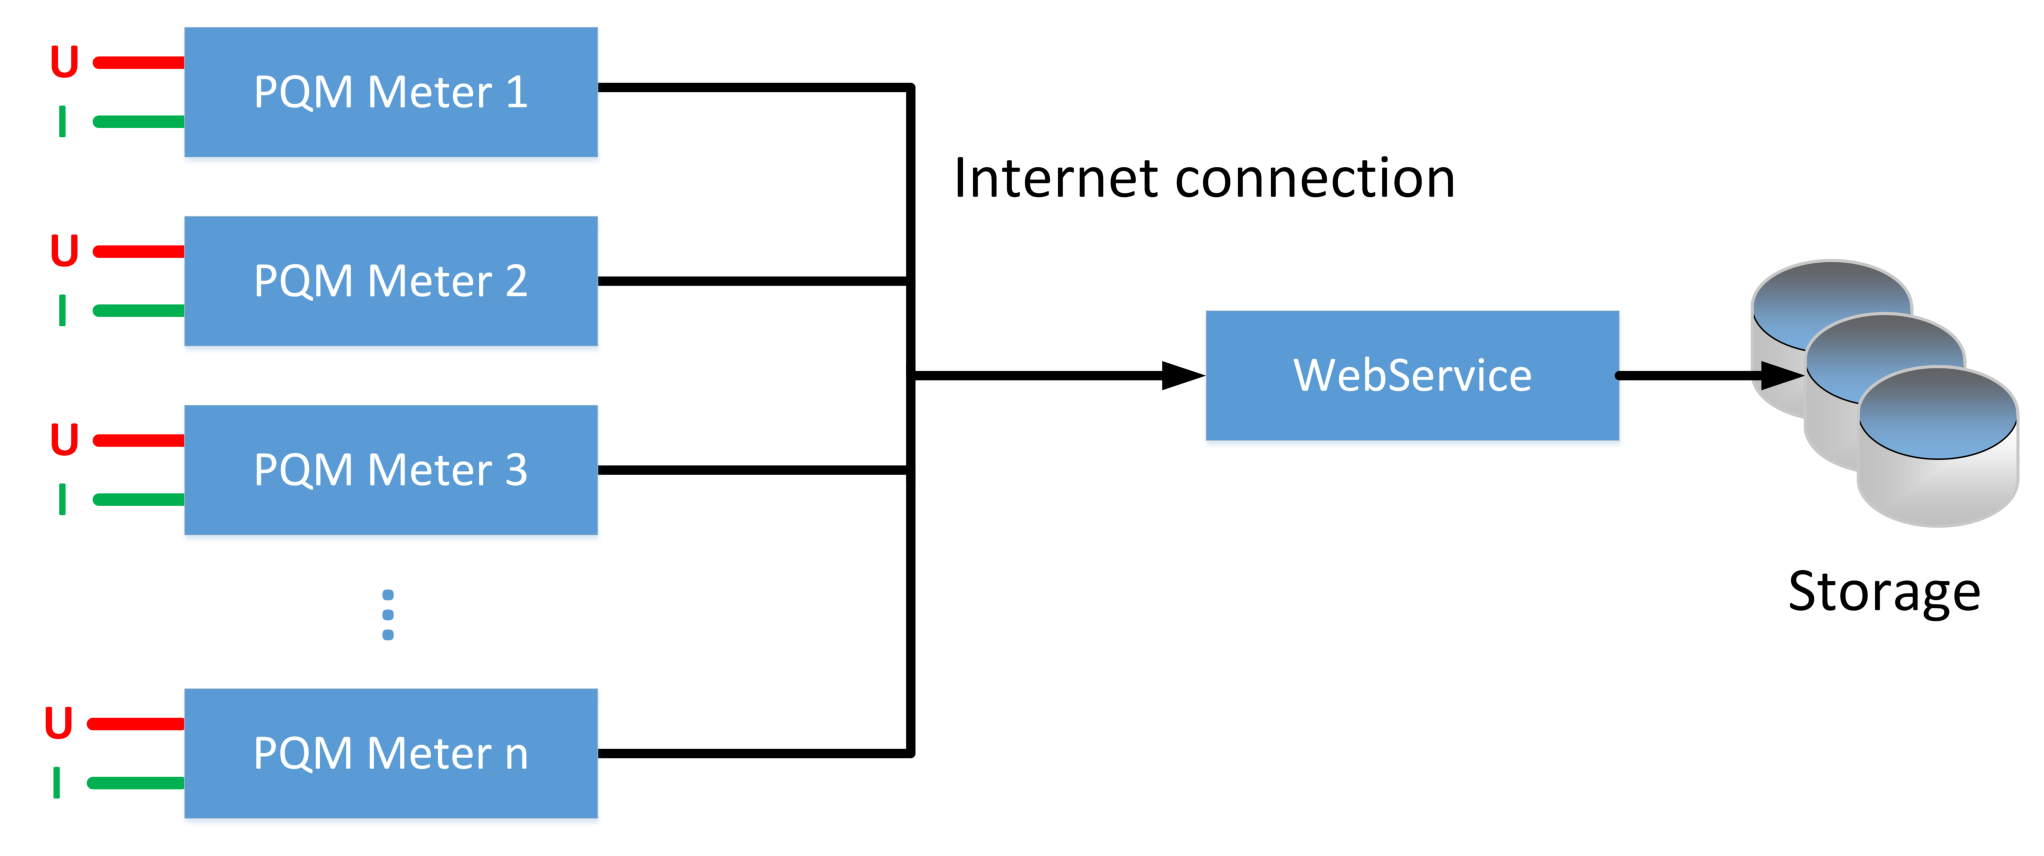
\includegraphics[scale=0.4]{graphics/simulation.eps}
	\caption{Simulation design}
	\label{fig:simulation_design}
\end{figure}

Different parameters of the simulation can be changed, such that different environments can be simulated and evaluated against each other. The following enumeration describes the parameters that can be adapted as input data to the simulation:

\begin{itemize}
	\item Bandwidth of the Internet connection
		\begin{itemize}
			\item Wired connection: 100 MB/s, 50 MB/s, 20 MB/s, 10 MB/s
			\item WiFi connection: 
			\item Cellphone connection: LTE (), 4G (), 2G (), GPRS ()
		\end{itemize}
	\item Number of PQM meters
	\item Number of Webservices
	\item Transmitted data
		\begin{itemize}
			\item Raw data
			\item Preprocessed data
		\end{itemize}
  \item Storage
		\begin{itemize}
			\item File archive
			\item SQL database (MySQL)
			\item NoSQL database (CrateDB)
		\end{itemize}		
\end{itemize}

Modifications of the above mentioned parameters have an effect to the following parts:

\begin{itemize}
	\item Server side storage
	\item Network load, network costs
	\item Server side throughput
\end{itemize}

The following table shows the expected results of the simulation:

% Please add the following required packages to your document preamble:
% \usepackage{multirow}
\begin{table}[h]
\centering
\begin{tabular}{l|c|c|c|c}
\hline
\multicolumn{1}{l|}{\multirow{2}{*}{\textbf{Parameter}}} & \multicolumn{1}{c|}{\multirow{2}{*}{\textbf{Modification}}} & \multicolumn{3}{c}{\textbf{Impact}}                                                                                                  \\ \cline{3-5} 
\multicolumn{1}{c|}{}                                    & \multicolumn{1}{c|}{}                                       & \multicolumn{1}{c|}{\textbf{Bandwidth}} & \multicolumn{1}{c|}{\textbf{Server side storage}} & \multicolumn{1}{c}{\textbf{Throughput}} \\ \hline \hline
\multirow{2}{*}{\textbf{Bandwidth}}                      & \nearrow                                                           & \nearrow                                       & -                                                 & -                                       \\ \cline{2-5} 
                                                         & \searrow                                                           & \searrow                                       & -                                                 & -                                       \\ \hline
\multirow{2}{*}{\textbf{Number of PQM meters}}           & \nearrow                                                           & \nearrow                                       & \nearrow                                                 & \searrow                                       \\ \cline{2-5} 
                                                         & \searrow                                                           & \searrow                                       & \searrow                                                 & \nearrow                                       \\ \hline
\multirow{2}{*}{\textbf{Number of Webservices}}          & \nearrow                                                           & -                                       & -                                                 & \nearrow                                       \\ \cline{2-5} 
                                                         & \searrow                                                           & -                                       & -                                                 & \searrow                                       \\ \hline
\multirow{2}{*}{\textbf{Transmitted Data}}               & \nearrow                                                           & \nearrow                                       & \nearrow                                                 & \searrow                                       \\ \cline{2-5} 
                                                         & \searrow                                                           & \searrow                                       & \searrow                                                 & \nearrow                                       \\ \hline
\multirow{3}{*}{\textbf{Server side storage}}            & File                                                        & -                                       & ?                                                 & -                                       \\ \cline{2-5} 
                                                         & SQL                                                         & -                                       & ?                                                 & -                                       \\ \cline{2-5} 
                                                         & NoSQL                                                       & -                                       & ?                                                 & -                                       \\ \hline
\end{tabular}
\caption{Simulation results}
\label{tab:SimulationResults}
\end{table}

\section{Evaluation}

\section{Impact on System Design}